% =========================================================================
%  FIT-ARCADE: A Transdisciplinary Architecture for Markerless,
%              Personalized Motion Exergaming  ---  10-PAGE SHORT VERSION
%  SDPS 2026 (Springer LNCS, llncs.cls)
%  Build: pdflatex main-short && bibtex main-short && pdflatex main-short x2
% =========================================================================
\documentclass[runningheads]{llncs}

\usepackage[T1]{fontenc}
\usepackage{graphicx}
\usepackage{amsmath,amssymb}
\usepackage{algorithm}
\usepackage[noend]{algpseudocode}
\usepackage{booktabs}
\usepackage{tabularx}
\usepackage{url}
\usepackage{hyperref}
\usepackage{marvosym} % \Letter (corresponding-author glyph)

\newcolumntype{L}[1]{>{\raggedright\arraybackslash}p{#1}}
\newcommand{\sys}{\textsc{FIT-ARCADE}}
\newcommand{\motionbus}{\texttt{MotionBus}}
\newcommand{\motionbridge}{\texttt{MotionBridge}}
\newcommand{\motionmap}{\texttt{MOTION\_MAP}}
\newcommand{\postmsg}{\texttt{postMessage}}
\newcommand{\citecompanion}{\cite{companion2026}}

\begin{document}

\title{FIT-ARCADE: A Transdisciplinary Architecture for Markerless, Personalized Motion Exergaming}

\author{%
  Sanket Salvi\textsuperscript{(\Letter)} \and
  Anuradha Nagare \and
  Anita Thengade \and
  Sagar Apune \and \\
  Mansi Sharma \and
  Vibhanshi Moon \and
  Ruchi Shukla%
}
\authorrunning{S. Salvi et al.}
\institute{Department of Computer Engineering and Technology, School of Computer
Science and Engineering, Dr.~Vishwanath Karad MIT World Peace University,
Pune, India\\
\email{sanket.salvi@mitwpu.edu.in} (corresponding author)\\
\email{\{anuradha.nagare, anita.thengade, sagar.apune,}\\
\email{mansi.sharma, vibhanshi.moon, ruchi.shukla\}@mitwpu.edu.in}}

\maketitle

\begin{abstract}
Exergames are a promising response to physical inactivity, yet existing platforms
are tightly coupled to specific sensors, engines, and exercise regimes, making them
hard to extend, personalize, or compose across the disciplines they span. We present
\sys{}, a browser-based, markerless motion-exergaming platform whose contribution is
a \emph{transdisciplinary seam architecture}: a layered, decoupled design that lets
six normally entangled disciplines---computer vision, control and personalization,
human--computer interaction, game design, exercise science, and software
engineering---co-evolve independently through stable interface contracts. Grounded in
Design Science Research, we derive design principles and instantiate them as a
single-camera pose layer, a normalized \motionbus{} event hub, per-game
\motionbridge{} translators, and engine-agnostic game integration via the browser
\postmsg{} protocol. Seven heterogeneous games across two engines (Phaser~3,
Three.js) and six exercise modalities run from one webcam with no wearables and no
change to their gameplay code. A formative evaluation shows engine-agnostic
extensibility and low seam latency (median $1.65$\,ms). Beyond the artifact, we distil
the seam into a \emph{reusable methodological contribution}---a transdisciplinary design
pattern and a Discipline$\times$Concern$\times$Design-Response planning tool that transfer
to other human-in-the-loop cyber-physical systems. The sensing and adaptation
subsystems are treated as black boxes here and evaluated in a companion
paper~\citecompanion{}.
\keywords{Transdisciplinary integration \and design science research \and
transdisciplinary design pattern \and software architecture \and human-in-the-loop
systems \and exergaming \and markerless motion capture \and engine-agnostic middleware.}
\end{abstract}

% =========================================================================
\section{Introduction}\label{sec:intro}
% =========================================================================
Physical inactivity is a leading risk factor for global mortality~\cite{who2022inactivity}.
Exergames---video games driven by vigorous bodily motion---elicit moderate-to-vigorous
activity comparable to conventional exercise and are effective, engaging
interventions across age groups~\cite{chen2023exergames}. Yet adoption is limited by
four barriers: (i)~\emph{sensor lock-in} to proprietary depth cameras or wearables;
(ii)~\emph{engine specificity}, with motion logic hard-wired into a single title;
(iii)~\emph{one-size-fits-all difficulty} that ignores individual effort and thus
breaks flow~\cite{csikszentmihalyi1990flow}; and (iv)~\emph{disciplinary
entanglement}---building an exergame simultaneously demands computer vision, game
design, exercise science, and interaction design, so a change in one discipline
cascades into all others~\cite{sinclair2007considerations}.

We argue the fourth barrier is the root cause of the first three: because the
disciplines are not compositionally separated, each system is rebuilt from scratch.
Through the SDPS lens this is a \emph{transdisciplinary integration}
problem~\cite{nicolescu2002manifesto,ertas2010transdisciplinary}---the challenge is
designing the \emph{interfaces} that let independently advancing disciplines compose.
Our insight is a \emph{motion seam}: a narrow, stable interface layer that decouples
the six contributing disciplines so each can evolve on its own. Realized as a layered
browser architecture in \sys{}, it turns heterogeneous keyboard games into
body-motion exergames using only a standard webcam.

\noindent\textbf{Contributions.} We frame this as a \emph{methodological/conceptual}
contribution. It offers (1)~a reusable \emph{transdisciplinary design pattern}---the
``motion seam''---with design principles (DP1--DP5) derived through Design Science
Research~\cite{hevner2004dsr}; (2)~a layered \emph{seam architecture} instantiating the
pattern, together with a Discipline$\times$Concern$\times$Design-Response \emph{planning
tool} (Table~\ref{tab:transmap}) for anticipating disciplinary boundaries; and (3)~a
formative evaluation over seven games and two engines. The sensing and
adaptive-personalization subsystems are black boxes here and evaluated
in~\citecompanion{}. \textbf{Research question:} \emph{how can a decoupled seam
architecture operationalize transdisciplinary integration in a markerless,
personalized exergaming system, and what reusable method does it yield?}

% =========================================================================
\section{Background and Related Work}\label{sec:related}
% =========================================================================
\textbf{Exergames and markerless sensing.} Exergames embed activity into gameplay so
players exercise as a side-effect of play; the Kinect era enabled skeleton tracking
but required depth sensors~\cite{sinclair2007considerations}. Recent RGB pose
estimators---MediaPipe Pose (BlazePose)~\cite{bazarevsky2020blazepose}---deliver
real-time 33-landmark skeletons in the browser, and validation studies confirm their
accuracy for movement analysis against marker-based
references~\cite{hii2023mediapipe}, removing the depth-camera/wearable requirement.

\textbf{Input abstraction and adaptation.} The game-architecture literature stresses
decoupling input from game logic~\cite{nystrom2014game}, but existing abstraction
layers target controllers, not whole-body motion, and no middleware normalizes pose
events across heterogeneous engines. The browser \postmsg{} API~\cite{html5postmessage}
offers a secure cross-origin transport for such a seam. Dynamic difficulty
adjustment~\cite{hunicke2005dda} modulates challenge to sustain
flow~\cite{sweetser2005gameflow}; heart rate is an objective effort measure, and
remote photoplethysmography (rPPG) recovers it from webcam
video~\cite{wang2017pos,debnath2025rppg}, closing a wearable-free loop---subsystems
detailed in~\citecompanion{}.

\textbf{Transdisciplinarity and the gap.} Transdisciplinarity seeks unity of knowledge
across disciplinary boundaries~\cite{nicolescu2002manifesto,ertas2010transdisciplinary};
Design Science Research (DSR)~\cite{hevner2004dsr,peffers2007dsrm} frames our
build--evaluate method. No existing exergaming platform (a)~decouples sensing from game
logic via a stable, engine-agnostic seam, (b)~supports multiple engines through one
interface, and (c)~frames this as a systematic transdisciplinary architecture. \sys{}
addresses this gap.

% =========================================================================
\section{Transdisciplinary Design Approach}\label{sec:approach}
% =========================================================================
Following DSR~\cite{hevner2004dsr,peffers2007dsrm} we identify the problem, derive
requirements, build the artifact (the seam architecture), and evaluate it formatively
(Sect.~\ref{sec:eval}). Table~\ref{tab:transmap} is the transdisciplinary blueprint:
each row is an independent axis of expertise whose design response must be realizable
without forcing changes in other rows.

\begin{table}[htbp]
\centering
\caption{Discipline $\times$ Concern $\times$ Design-Response (transdisciplinary map).}
\label{tab:transmap}
\footnotesize
\begin{tabularx}{\textwidth}{@{}L{2.5cm}L{3.7cm}L{5.6cm}@{}}
\toprule
\textbf{Discipline} & \textbf{Key concern} & \textbf{Design response in \sys{}} \\
\midrule
Computer vision & Real-time pose from RGB; model updates & Single-camera \texttt{PoseDetector}; new models plug in without changing games \\
Control \& personalization & Effort estimation; adaptive difficulty & Black-box \texttt{EffortEstimator}$+$\texttt{DifficultyController}; output is one scalar sent via the seam \\
HCI \& coaching & Move discoverability; feedback & \texttt{Coach} cues $+$ \texttt{MoveDemo} stick figure; spoken prompts \\
Game design \& engines & Diverse genres; 2D/3D engines & Engine-agnostic \motionbridge{} $+$ per-game \motionmap{}; keyboard logic intact \\
Exercise science & Modality variety; progressive overload & Seven games, six modalities; phased work/rest circuit; rep tracking \\
Software engineering & Modularity; latency; deployment & Layered design; \postmsg{} seam; \texttt{localStorage} persistence; zero-install browser \\
\bottomrule
\end{tabularx}
\vspace{-0.4em}
\end{table}

\noindent\textbf{Design principles.} \textbf{DP1 Single-camera ownership:} exactly one
component owns the camera and ML model; all others receive derived data.
\textbf{DP2 Normalized event abstraction:} the \motionbus{} converts continuous posture
into discrete, debounced events and hold states, decoupling pose semantics from game
input. \textbf{DP3 Minimal-touch bridge:} each game declares a \motionmap{} onto its
\emph{existing} keys; the bridge synthesizes native events and never edits gameplay
code. \textbf{DP4 Cross-origin seam:} games run in iframes; all communication flows
through \postmsg{}, enforcing isolation and engine independence. \textbf{DP5 Black-box
sensing/adaptation:} rPPG and adaptive difficulty are encapsulated behind scalar
interfaces (\texttt{bpm}, \texttt{effort}, \texttt{difficulty}), replaceable
independently.

% =========================================================================
\section{System Architecture}\label{sec:arch}
% =========================================================================
\begin{figure}[htbp]
  \centering
  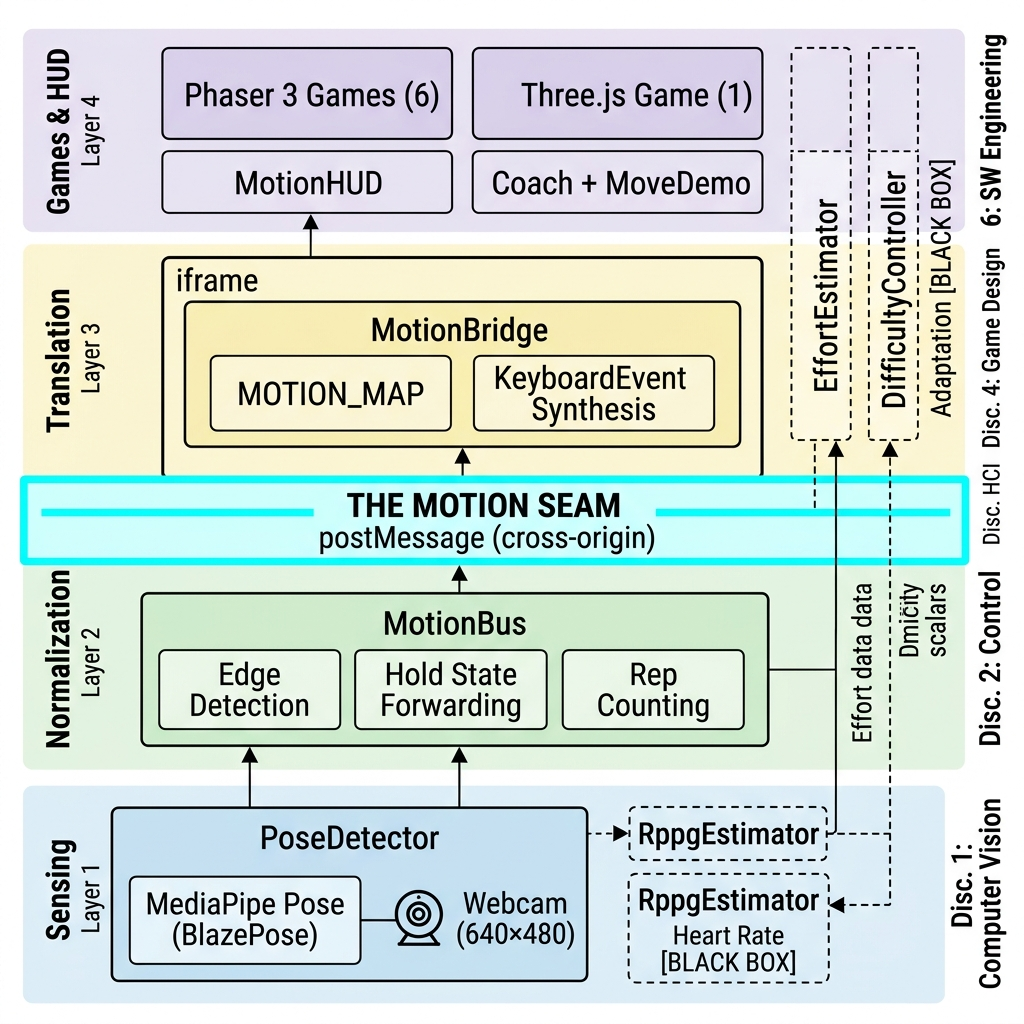
\includegraphics[width=0.8\textwidth]{figures/architecture}
  \caption{Layered architecture. The motion seam
  (\motionbus{}$\to$\postmsg{}$\to$\motionbridge{}) is the stable interface that
  decouples the six disciplines; sensing and adaptation (dashed) are black boxes.}
  \label{fig:arch}
  \vspace{-0.6em}
\end{figure}

Figure~\ref{fig:arch} shows four layers traversed each frame. \textbf{(1)~Sensing (DP1).}
A \texttt{PoseDetector} singleton runs MediaPipe Pose (BlazePose,
$640{\times}480$)~\cite{bazarevsky2020blazepose} and emits a \emph{posture} record: Boolean
gesture flags (\texttt{isJumping}, \texttt{isSquatting}, \texttt{isLeaningLeft},
\texttt{isPunchingLeft}, \dots) and continuous values. The rPPG heart-rate estimator
piggybacks on the same frames; its output feeds the HUD and effort modules (internals
in~\citecompanion{}). \textbf{(2)~Normalization (DP2).} The \motionbus{} performs
per-frame edge detection of discrete events, forwards hold states, counts reps, and
posts a slim \texttt{\{posture, events\}} payload to the active game iframe.
\textbf{(3)~The seam (DP3, DP4).} Inside each iframe the \motionbridge{} translates the
payload into native \texttt{KeyboardEvent}s per the game's \motionmap{}; \emph{tap} and
\emph{hold} mappings are supported. This is the \emph{only} addition to a game: a
\motionmap{} object and two \texttt{<script>} tags. \textbf{(4)~Games and HUD.} Games are
standalone HTML running unmodified input logic; a \texttt{MotionHUD} overlays telemetry.
The adaptation layer fuses rep cadence and heart-rate reserve into an effort signal and
emits a scalar \texttt{MOTION\_DIFFICULTY} $\in[0.85,1.2]$ that games read to scale
obstacle speed---both pluggable without touching any game.

\textbf{Engine agnosticism.} Two engines coexist behind one seam:
Phaser~3~\cite{phaser2023} (six games, 2D Canvas/WebGL, including a pseudo-3D lane
runner) and Three.js~\cite{threejs2023} (a real-3D WebGL lane runner with GLTF models).
From the seam's view both are opaque iframes consuming identical events, demonstrating
that engine choice is a private decision of the game-design discipline.

% =========================================================================
\section{Core Mechanisms}\label{sec:mech}
% =========================================================================
\textbf{Pose-to-virtual-input synthesis.} The \motionbus{} converts posture Booleans
into discrete events by per-field rising-edge detection:
\begin{equation}
  \text{event}(e)=\text{fire}(e)\ \text{iff}\ \texttt{posture}[f_e]_{t}\land\lnot\,\texttt{posture}[f_e]_{t-1},
  \label{eq:edge}
\end{equation}
where $f_e$ is the posture field mapped to event $e$ (e.g.\ $f_{\texttt{jump}}=\texttt{isJumping}$).
The \motionbridge{} then synthesizes keys. A critical detail is the \emph{keyCode
override}: since \texttt{KeyboardEvent.keyCode} is read-only yet Phaser~3.55 reads it
for input dispatch, the bridge uses \texttt{Object.defineProperty(e,'keyCode',\{get:()=>k\})}.
For \emph{tap} mappings a keydown is dispatched and a keyup follows after
$120$\,ms---long enough for Phaser's \texttt{JustDown()} to register within one update
cycle; \emph{hold} mappings toggle keydown/keyup with the posture flag
(Algorithm~\ref{alg:pose2input}).

\begin{algorithm}[htbp]
\caption{Pose-to-virtual-input synthesis}\label{alg:pose2input}
\begin{algorithmic}[1]
\Procedure{OnPose}{$\mathit{posture}$} \Comment{hub side}
  \State $\mathit{events}\gets[]$
  \For{$(e,f_e)\in\texttt{edgeMap}$}
    \If{$\mathit{posture}[f_e]\land\lnot\,\texttt{prev}[f_e]$}
      \State $\mathit{events}.\text{push}(e)$; \Call{Emit}{$e$}; \textbf{if} $e\in\texttt{repEvents}$ \textbf{then} $\texttt{reps}{+}{+}$
    \EndIf
    \State $\texttt{prev}[f_e]\gets\mathit{posture}[f_e]$
  \EndFor
  \State \Call{PostToGame}{\texttt{\{posture, events\}}}
\EndProcedure
\Procedure{OnReceive}{$\mathit{posture},\mathit{events}$} \Comment{bridge side}
  \For{$e\in\mathit{events}$}
    \If{$\texttt{MAP}[e].\text{type}=\texttt{'tap'}$} \Call{Tap}{$\texttt{MAP}[e]$} \Comment{keydown; keyup after $120$\,ms} \EndIf
  \EndFor
  \For{$(e,\mathit{def})\in\texttt{MAP}$ \textbf{with} $\mathit{def}.\text{type}=\texttt{'hold'}$}
    \State \Call{SetHeld}{$\mathit{def},\ \mathit{posture}[\mathit{def}.\text{state}]$}
  \EndFor
\EndProcedure
\end{algorithmic}
\end{algorithm}

\textbf{Procedural pseudo-3D projection.} \emph{Hoverboard Alley} (2D Phaser) shows that
rich 3D depth is achievable in a 2D engine via $1/z$ projection. With a vanishing point
$(V_x,V_y)$ and object depth $z\in[z_{\text{near}},z_{\text{far}}]=[1,13]$:
\begin{align}
  s(z)=\tfrac{z_{\text{near}}}{z},\quad
  x_{\text{scr}}=V_x+(\ell-1)L_{\text{spread}}\,s(z),\quad
  y_{\text{scr}}=V_y+(Y_{p}-V_y)\,s(z),
  \label{eq:proj}
\end{align}
where $\ell\in\{0,1,2\}$ is the lane, $L_{\text{spread}}=250$, and $Y_p=505$ is the
hero's screen-$y$. A pooled spawner recycles sprites (no GC churn), advancing each object
by $\delta z=v_{\text{base}}\cdot D\cdot\Delta t$ ($D=\texttt{MOTION\_DIFFICULTY}$) and
recycling at $z\le z_{\text{recycle}}$. A lane-safety rule guarantees a survivable path:
\begin{equation}
  |\mathcal{B}_w|\le|\mathcal{L}|-1,
  \label{eq:lanesafe}
\end{equation}
i.e.\ the blocked-lane set $\mathcal{B}_w$ never covers all lanes
$\mathcal{L}=\{0,1,2\}$; a collectible spawns in a free lane with probability $0.6$.

\textbf{Coaching broadcast.} When a game's logic determines a move is needed it calls
\texttt{Coach.cue('JUMP!')}, which (i)~shows a pixel-font overlay, (ii)~speaks the move
once, and (iii)~posts \texttt{\{expectMove:$m$\}} to the hub, where $m$ is inferred from
the cue text. The hub's \texttt{MoveDemo} renders a looping neon stick figure of $m$ from
a 13-joint base skeleton with per-move parametric deformations over loop phase
$p\in[0,1]$ (e.g.\ \texttt{jump} offsets all joints by $-0.15\sin(\pi p)$). The pipeline is
unidirectional---games produce cues, the hub consumes them---so coaching is added without
touching game code.

% =========================================================================
\section{Implementation and Formative Evaluation}\label{sec:eval}
% =========================================================================
\sys{} is a static web app with no server dependencies: MediaPipe Pose, Phaser~3.55 and
Three.js~0.147 from CDN, \postmsg{} transport, and \texttt{localStorage} persistence.
The hub is $\approx$2{,}800~lines across ten JavaScript modules; each game is a standalone
HTML file. Table~\ref{tab:games} lists the seven games. Figure~\ref{fig:ingame} shows the
shared neon stage---marquee HUD, the \emph{DO THIS MOVE} \texttt{MoveDemo} box, the live
\emph{YOU$\cdot$TRACKING} camera box, and the \emph{HOW TO PLAY} rail---across two engines.

\begin{table}[htbp]
\centering
\caption{The seven \sys{} games.}
\label{tab:games}
\footnotesize
\begin{tabularx}{\textwidth}{@{}L{2.4cm}L{2.0cm}L{3.0cm}L{1.4cm}L{2.6cm}@{}}
\toprule
\textbf{Game} & \textbf{Target} & \textbf{Motion} & \textbf{Engine} & \textbf{Pattern} \\
\midrule
Rooftop Runner & Legs/cardio & Jump, Squat & Phaser & Side-scroll dodge \\
Neon Wall Climber & Shoulders/lats & Jump, Punch L/R & Phaser & Vertical climb \\
Industrial Rope & Core & Jump, Lean L/R & Phaser & Vertical climb \\
Street Brawler & Arms & Punch L/R, Squat & Phaser & Side-scroll fight \\
Cyber-Train Crawl & Chest/triceps & Push-up, Squat & Phaser & Side-scroll dodge \\
Jetpack Ascent & Shoulders/aerobic & Arms overhead & Phaser & Altitude control \\
Hoverboard Alley & Obliques/core & Lean L/R & Three.js & 3-lane runner \\
\bottomrule
\end{tabularx}
\vspace{-0.4em}
\end{table}

\begin{figure}[htbp]
  \centering
  \newcommand{\ingamepanel}[2]{%
    \IfFileExists{#1}{\includegraphics[width=0.32\textwidth]{#1}}%
    {\fbox{\parbox[c][2.4cm][c]{0.30\textwidth}{\centering\footnotesize [screenshot] #2}}}}
  \ingamepanel{figures/ingame-rooftop.jpg}{Rooftop (2D)}\hfill
  \ingamepanel{figures/ingame-jetpack.jpg}{Jetpack (2D)}\hfill
  \ingamepanel{figures/ingame-hoverboard.jpg}{Hoverboard (3D)}
  \caption{Three in-game views sharing one motion seam: \texttt{MoveDemo} cue (left),
  neon stage with marquee HUD (centre), live camera/skeleton and \emph{HOW TO PLAY}
  rail (right). Rooftop/Jetpack are Phaser~3; Hoverboard Alley is Three.js (real 3D). The
  retro game visual assets shown were generated using Google Gemini.}
  \label{fig:ingame}
  \vspace{-0.6em}
\end{figure}

\textbf{E1 Extensibility.} To motion-ify a keyboard game a developer (i)~declares a
\motionmap{}, (ii)~includes \texttt{motion-bridge.js} and \texttt{coach.js}, and
(iii)~optionally adds \texttt{Coach.cue()} calls and reads \texttt{MOTION\_DIFFICULTY}.
Across all seven games the \motionmap{} has 2--3 entries and \emph{zero} lines of original
gameplay code were modified; bridge$+$coach total $\approx$230~shared LOC.

\textbf{E2 Engine agnosticism.} Phaser~3 (2D) and Three.js (3D) operate behind the same
\motionbridge{}; the \postmsg{} transport carries only JSON-safe posture, so a third
engine needs only a \motionmap{} and two script tags---no hub changes.

\textbf{E3 Seam latency.} We measured one-way seam transport (hub \postmsg{} send to
in-iframe receipt, just before \texttt{KeyboardEvent} synthesis) with an echo probe and
\texttt{performance.now()} timestamps, \emph{while a Phaser game rendered
concurrently}. Over $N{=}600$ samples: median $1.65$\,ms, mean $2.29$\,ms, p95
$6.05$\,ms, max $8.6$\,ms (Fig.~\ref{fig:latency}). Even the tail is well within the
$16.7$\,ms 60\,fps frame budget, confirming the seam does not perceptibly degrade
responsiveness. This isolates the transport; upstream MediaPipe inference is a property
of the sensing black box~\citecompanion{}.

\begin{figure}[htbp]
  \centering
  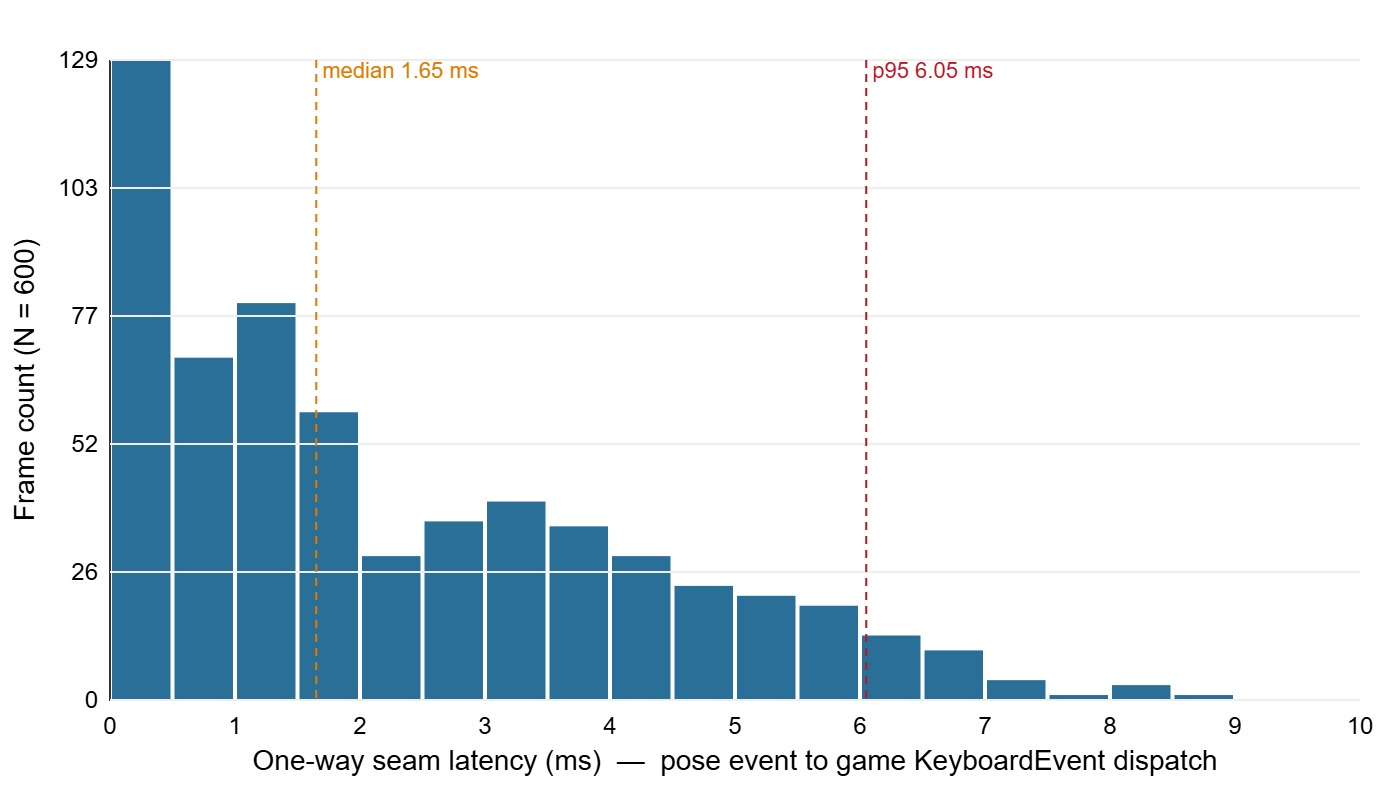
\includegraphics[width=0.72\textwidth]{figures/latency.jpg}
  \caption{One-way motion-seam latency over $N{=}600$ frames measured with a Phaser game
  rendering concurrently. Median $1.65$\,ms; p95 $6.05$\,ms.}
  \label{fig:latency}
  \vspace{-0.6em}
\end{figure}

\textbf{E4 Design-principle walkthrough.} Each DP is met by concrete evidence: only
\texttt{PoseDetector} calls \texttt{getUserMedia} (DP1); six discrete events plus ten hold
states are exposed and games never parse landmarks (DP2); all games run with zero
gameplay edits (DP3); two engines coexist with independent load/unload (DP4); rPPG and the
difficulty controller each expose one scalar, so internal replacement affects no game (DP5).
Efficacy and user studies are the companion paper's scope~\citecompanion{}.

% =========================================================================
\section{Discussion and Conclusion}\label{sec:disc}
% =========================================================================
The seam concretely enables independent disciplinary evolution: the vision model can be
swapped (only \texttt{PoseDetector} changes), rPPG sensing was added late as a listener,
the Three.js game was integrated with a two-entry \motionmap{}, the difficulty controller
could become a learning agent behind the same scalar, and coaching was plugged in through
the \texttt{expectMove} message---each a different discipline, none touching the others.
As the paper's transferable \emph{methodological contribution}, three principles
generalize beyond exergaming to transdisciplinary human-in-the-loop systems:
\emph{seam-first design} (identify discipline boundaries before implementation;
Table~\ref{tab:transmap} is a reusable planning tool), \emph{translate, don't modify}
(adapt an artifact's native interface rather than editing its internals), and
\emph{scalar contracts at boundaries} (reduce internal state to minimal signals such as
effort $\in[0,1]$).

\textbf{Limitations.} The formative evaluation is author-conducted; all games are authored
in-house, so third-party integration would more strongly test DP3; latency was measured on
one desktop; and sensing accuracy is out of scope (evaluated in~\citecompanion{}).

\textbf{Conclusion.} \sys{} shows that a decoupled \emph{transdisciplinary seam
architecture}---normalized events, translation bridges, and scalar contracts---lets six
disciplines co-evolve independently while composing into a coherent, markerless,
personalized exergaming system. Its value lies not in any subsystem but in the stable
interfaces that operationalize the transdisciplinary integration SDPS advocates. The
reusable design pattern, the Discipline$\times$Concern$\times$Design-Response planning
tool, and the three generalizable principles are the paper's methodological takeaway,
transferable beyond exergaming to other transdisciplinary human-in-the-loop systems.
Future work includes empirical user studies~\citecompanion{}, more engines, and
multi-player motion exergaming.

\subsubsection*{Disclosure of Generative-AI Use.}
The retro game visual assets displayed in this paper (e.g., Fig.~\ref{fig:ingame}) were
generated using Google Gemini. The authors reviewed all such assets and take full
responsibility for the content of this paper.

\bibliographystyle{splncs04}
\bibliography{references-short}
\end{document}
